\documentclass[
  bibliography=totoc,     % Literatur im Inhaltsverzeichnis
  captions=tableheading,  % Tabellenüberschriften
  titlepage=firstiscover, % Titelseite ist Deckblatt
]{scrartcl}

%irgendetwas mit Tabelen und Figuren anders Nummerieren 
\usepackage{chngcntr}
\usepackage{longtable} 

\usepackage{titling}

%Textdatein einfügen
\usepackage{verbatim}

% Paket float verbessern
\usepackage{scrhack}

% Warnung, falls nochmal kompiliert werden muss
\usepackage[aux]{rerunfilecheck}

% unverzichtbare Mathe-Befehle
\usepackage{amsmath}
% viele Mathe-Symbole
\usepackage{amssymb}
% Erweiterungen für amsmath
\usepackage{mathtools}

% Fonteinstellungen
\usepackage{fontspec}
% Latin Modern Fonts werden automatisch geladen
% Alternativ zum Beispiel:
%\setromanfont{Libertinus Serif}
%\setsansfont{Libertinus Sans}
%\setmonofont{Libertinus Mono}

% Wenn man andere Schriftarten gesetzt hat,
% sollte man das Seiten-Layout neu berechnen lassen
\recalctypearea{}

% deutsche Spracheinstellungen
\usepackage[ngerman]{babel}


\usepackage[
  math-style=ISO,    % ┐
  bold-style=ISO,    % │
  sans-style=italic, % │ ISO-Standard folgen
  nabla=upright,     % │
  partial=upright,   % ┘
  warnings-off={           % ┐
    mathtools-colon,       % │ unnötige Warnungen ausschalten
    mathtools-overbracket, % │
  },                       % ┘
]{unicode-math}

% traditionelle Fonts für Mathematik
\setmathfont{Latin Modern Math}
% Alternativ zum Beispiel:
%\setmathfont{Libertinus Math}

\setmathfont{XITS Math}[range={scr, bfscr}]
\setmathfont{XITS Math}[range={cal, bfcal}, StylisticSet=1]

% Zahlen und Einheiten
\usepackage[
  locale=DE,                   % deutsche Einstellungen
  separate-uncertainty=true,   % immer Unsicherheit mit \pm
  per-mode=symbol-or-fraction, % / in inline math, fraction in display math
]{siunitx}

\DeclareSIUnit{\channel}{Channel}
\DeclareSIUnit{\year}{a}

% chemische Formeln
\usepackage[
  version=4,
  math-greek=default, % ┐ mit unicode-math zusammenarbeiten
  text-greek=default, % ┘
]{mhchem}

% richtige Anführungszeichen
\usepackage[autostyle]{csquotes}

% schöne Brüche im Text
\usepackage{xfrac}

% Standardplatzierung für Floats einstellen
\usepackage{float}
\floatplacement{figure}{htbp}
\floatplacement{table}{htbp}

% Floats innerhalb einer Section halten
\usepackage[
  section, % Floats innerhalb der Section halten
  below,   % unterhalb der Section aber auf der selben Seite ist ok
]{placeins}

% Seite drehen für breite Tabellen: landscape Umgebung
\usepackage{pdflscape}

% Captions schöner machen.
\usepackage[
  labelfont=bf,        % Tabelle x: Abbildung y: ist jetzt fett
  font=small,          % Schrift etwas kleiner als Dokument
  width=0.9\textwidth, % maximale Breite einer Caption schmaler
]{caption}
% subfigure, subtable, subref
\usepackage{subcaption}

% Grafiken können eingebunden werden
\usepackage{graphicx}
\usepackage{wrapfig}

% schöne Tabellen
\usepackage{booktabs}
\usepackage[table]{xcolor}

% Verbesserungen am Schriftbild
\usepackage{microtype}

% Literaturverzeichnis
\usepackage[
  backend=biber,
  sorting=none
]{biblatex}
% Quellendatenbank
\addbibresource{lit.bib}
\addbibresource{programme.bib}

% Hyperlinks im Dokument
\usepackage[
  german,
  unicode,        % Unicode in PDF-Attributen erlauben
  pdfusetitle,    % Titel, Autoren und Datum als PDF-Attribute
  pdfcreator={},  % ┐ PDF-Attribute säubern
  pdfproducer={}, % ┘
]{hyperref}
% erweiterte Bookmarks im PDF
\usepackage{bookmark}

% Trennung von Wörtern mit Strichen
\usepackage[shortcuts]{extdash}

%\setcounter{tocdepth}{3} % + subsubsections



\author{%
  Benedikt Lütke Lanfer \\%
  \href{mailto:benedikt.luetkelanfer@tu-dortmund.de}{benedikt.luetkelanfer@tu-dortmund.de}%
  \and%
  Enno Wellmann \\%
  \href{mailto:enno.wellmann@tu-dortmund.de}{enno.wellmann@tu-dortmund.de}%
}
\publishers{TU Dortmund – Fakultät Physik}


\newcommand*\diff{\mathop{}\!\mathrm{d}}

\NewDocumentCommand \OverfullCenter {+m} {
\noindent\makebox[\linewidth]{#1} }

\usepackage{adjustbox}


% %Tabellen und Figuren Einstellung
% \counterwithout{table}{section}
% \counterwithout{figure}{section}
% \renewcommand{\thetable}{\Roman{table}}
% \renewcommand{\thefigure}{\Roman{figure}}

%Richtiges Einrücken
\setlength{\parindent}{0pt}


\title{V64: Modern Interferometry}
\author{Benedikt Lütke Lanfer \and Enno Wellmann}
\date{27. Mai 2024}
\publishers{TU Dortmund – Fakultät Physik}

\begin{document}
\begin{titlingpage}
    \begin{center}
        \begin{Huge}
            \textbf{\thetitle\\}
        \end{Huge}
    \end{center}
    \vspace{4cm}
    
\includegraphics[width=\textwidth]{Bilder/Logo_TU.png} \\
    \vspace{4cm}
    \begin{center}
        \begin{huge}
            \theauthor\\
        \end{huge}
        \vspace{0.5cm}
        \begin{Large}
            benedikt.luetkelanfer@tu-dortmund.de\\
            enno.wellmann@tu-dortmund.de\\
            \vspace{1.4cm}
            Bearbeitet: \today\\
            Durchgeführt: \thedate\\
            TU Dortmund – Fakultät Physik\\
        \end{Large}
    \end{center}
\end{titlingpage}
\tableofcontents
\newpage
%Shortcuts
\let\t\text\

% \section{Vorbereitung}
$\Delta t_c  = 1/ \Delta \nu$
Kohärenzzeit ist die Zeitspanne in der man die Phase der Lichtwelle noch vorhersagen kann
Erzeigung von Interferenzmustern ist ein gutes Maß für Kohärenz.
Interferenztherm
$E^2 = (E_1 +E_2)^2$

$$I_{12} = E_{01}E_{02}cos{\delta} = 2 \sqrt{I_1 I_2} \cos{\delta}$$
$\delta = (k_1 r- k_2 r + \epsilon_1-\epsilon_2)$
Auslöschung bei $\delta= 0, \pm 2\pi,\pm4\pi,\dots$

Lorenz-Lorentz-Gesetz
Annäherung für Gase:
$$n \simeq \sqrt{1 + \frac{3A_p}{R T}} $$
\section{Objective}
Goal of this Experiment is to learn the function of a Sagnac Interferometer and
to measure its contrast as well as the refractive index of glass and air,
dependent of the pressure.

%---------------------------------------------------------------------------------------------------------------------------------------------------------------%

\section{Theory}
In the experiment a Helium-Neon-Laser, which emits linear polarized coherent
light, is used in a Sagnac Interferometer. To understand the experiment
properly the following theory will explain the necessary technical terms as
well as the used setup.

\subsection{Coherence}
Coherence describes weather light is temporally or spatial in Phase. If light
is temporally coherent than its Phase difference is constant for a time period
$\Delta t_c$, equally if light is spatial coherent than its Phase difference is
constant in a limited space. As a result of superimposing two coherent waves,
spatial and temporally Interference can be observed.

\subsection{Polarization}
Another characteristic of light is its polarization, which describes the
geometrical orientation of the oscillations of the light. Light consists of
perpendicular oscillating electric and magnetic fields. Normally for
polarization only one field oscillations is depicted for simplicity, because
the fields always stands perpendicular to each other and therefore have the
same polarization. The three common polarization types are

\begin{enumerate}
	\item linear polarization: oscillations on a line
	\item circular polarization: oscillations on a circle
	\item elliptic polarization: oscillations on an ellipse
\end{enumerate}

which are better shown in the following graphic

\begin{figure}[H]
	\centering
	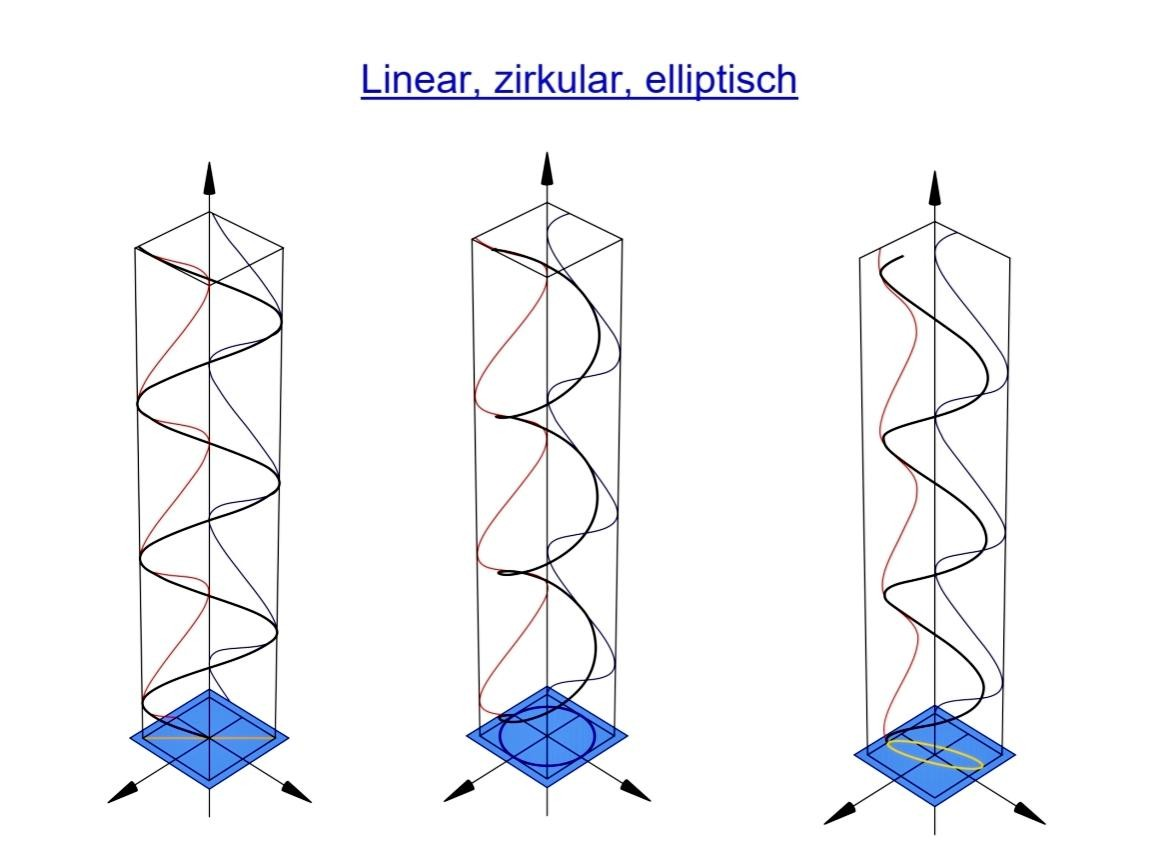
\includegraphics[width=\textwidth]{Bilder/Polarization.png}
	\caption{Polarization types \cite{...}}\label{fig:po}
\end{figure}

The polarization influences weather interference pattern occur or not. To be
able to observe interference the waves have to be coherent and have the same
polarization. In the following experiment only linear polarized light is used.
To change the direction of oscillation of the linear light a polarization
filter, which only lets light oscillating in one direction trough, can be used.
If linear light oscillating in an angle $\alpha $ to the polarization filter,
the intensity of the light decreases by

\begin{equation}
	I=I_0 \cdot \cos^2(\alpha )
	\label{eq:pol}
\end{equation}

after passing the filter.

\subsection{Refractive Index}
The refractive index $n$ describes the velocity of the light in matter

\begin{equation}
	c_m=\frac{c}{n}
\end{equation}

compared to constant vacuum velocity $c$. Also,, the phase of the light change
in matter by constant phase $\varphi $.

\subsubsection{Refractive index of glass}
To estimate the refractive index of glass in the experiment two rotatable glass
planes get inserted in the light beam. Each of the plane changes the phase of
the light dependent of the rotation angel $\theta $ by

\begin{equation}
	\Delta \varphi(\theta ) =\frac{2\pi }{\lambda_{vac}}T \cdot \left(\frac{n-1}{2n}\theta ^2 +O(\theta ^4)  \right)
\end{equation}

With the wavelength of the laser $\lambda_{vac}$ and the thickness $T$.
Together the two glass planes, which are each tilted by $\varphi_0=\pm 10°$,
change the phase by

\begin{align}
	\Delta \varphi(\theta ) & =\frac{2\pi T}{\lambda_{vac}} \frac{n-1}{2n} \cdot \left[(\theta+\varphi_0)^2 - (\theta-\varphi_0)^2 +O(\theta ^4)  \right] \notag \\
	                        & =\frac{4\pi T}{\lambda_{vac}} \frac{n-1}{n} \cdot \theta\varphi_0 +O(\theta ^4)
\end{align}\label{eq:glass}

The phase shift is connected to the number of interference maxima and minima by

\begin{equation}
	M=\frac{\Delta \varphi(\theta)}{2\pi}
\end{equation}

\subsubsection{Refractive index of gas}
To determine the refractive index of gas a pressure control tube of the gas is
inserted in the beam. The refractive index of gas is dependent of the
temperature $T$ and the pressure $p$ of the gas by the Lorentz-Lorenz-Law

\begin{equation}
	\frac{n^2-1}{n^2+1}=\frac{Ap}{RT}
\end{equation}

were $R$ is the gas constant and $A$ is the molar refractive. Also, the light
phase is shifted in the tube of length $L$ by

\begin{equation}
	\Delta \varphi(\theta ) =\frac{2\pi }{\lambda_{vac}}\Delta n L
\end{equation}

\subsection{Contrast}
The contrast of an interferometer

\begin{equation}
	C=\frac{I_{max}-I_{min}}{I_{max}+I_{min}}
	\label{eq:contrast}
\end{equation}

describes the normalized difference in the maximal intensity $I_{max}$ and the
minimal intensity $I_{min}$ and therefore $C \in [0,1] $. The superposition of
two waves with electric field components $E_1$, $E_2$ and a phase shift
$\varphi $ result in an intensity of

\begin{equation}
	I\varpropto \langle |E_1 \cos(\omega t) + E_2 \cos(\omega t+\varphi ) | \rangle
\end{equation}.

In the experiment the laser beam is split in two, therefore the absolute value
squared of the electric field components of the two waves add up to the laser
intensity $I_{laser}=E_1^2+E_2^2$. Furthermore, they only different in there
polarization orientation and not in there amplitude, so you can write

\begin{align*}
	E_1 & =\sqrt{\frac{I_{laser}}{2}} \cdot \cos(\phi ) \\
	E_2 & =\sqrt{\frac{I_{laser}}{2}} \cdot \sin(\phi )
\end{align*}

which result in

\begin{equation}
	I_{\frac{max}{min}}\varpropto I_{laser}\cdot [1\pm 2\cos(\phi )\sin(\phi )]
\end{equation}

Finally, inserting this in the formula for the contrast \eqref{eq:contrast}
yield

\begin{equation}
	C=\sin(2\phi )
\end{equation}

\subsection{Error calculation}
For error calculation, all \textbf{mean values} of N measurements are
calculated as follows:

\begin{equation}
	\overline{x} = \frac{1}{N} \cdot \sum_{i=1}^N x_i
	\label{eqn:Mittelwert}
\end{equation}

and all \textbf{standard deviations of the mean} with:

\begin{equation}
	\increment\overline{x} = \sqrt{\frac{1}{N\cdot(N-1)}\cdot\sum_{i=1}^N (x_i-\overline{x})^2}
	\label{eqn:St_Mittelwert}
\end{equation}

The error for correlated measurements is then calculated using the
\textbf{Gaussian error propagation}:

\begin{equation}
	\increment{f} = \sqrt{ \sum_{i = 1}^{N}  \biggl(\frac{\partial{f}}{\partial{x_i}}\biggr)^2\cdot(\increment{x_i})^2}
	\label{eqn:Gauss}
\end{equation}

Error propagation is determined using the Uncertainties \cite{uncertainties}
package in Python.

%---------------------------------------------------------------------------------------------------------------------------------------------------------------%

\section{Experimental Procedure}
\subsection{Setup Sagnac-Interferometer}
In the experiment a Sagnac-Interferometer is used in the following setup

\begin{figure}[H]
	\centering
	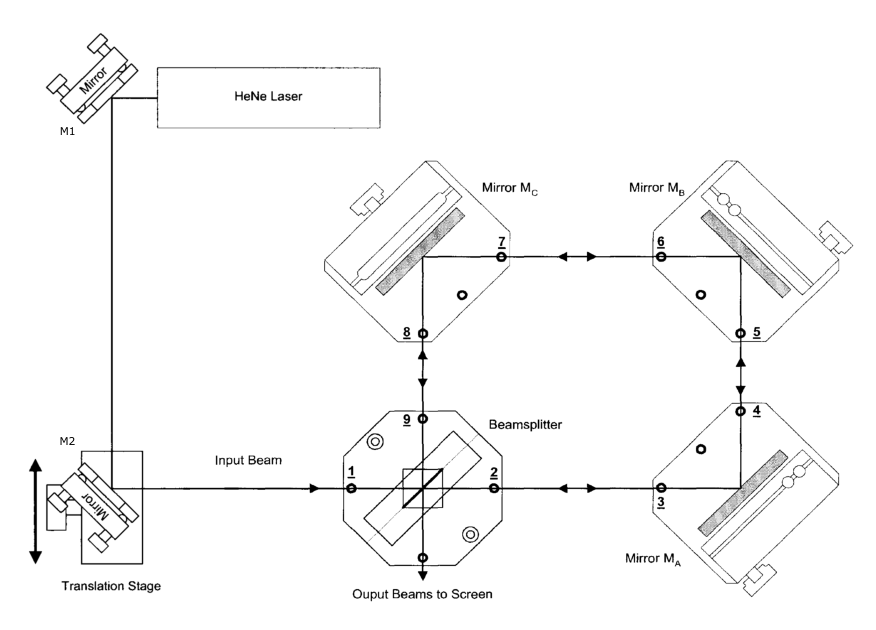
\includegraphics[width=\textwidth]{Bilder/Aufbau.png}
	\caption{Polarization types \cite{man:v64}}\label{fig:Aufbau}
\end{figure}

Form the HeNe-Laser the beam, with wavelength $\qty{632.990}{\nano\meter}$,
goes through a polarization filter were its polarization direction can be set
\eqref{eq:pol}. After this the beam goes in the polarizing beam splitter cube
(PBSC), where it gets split $90°$ and two overlapping beams go around the setup
in opposite direction. Until there are recombined in the PBSC and interfere
with each other. To fine tune the interferometer each mirror can be adjusted
either horizontal or vertical, which will be described later in the alignment
chapter. Furthermore, the mirror two can be rotated so that the light does not
hit the cube perfectly in the middle and therefore the two beams are separate
parallel beams and not overlapping. One of the beams can now be manipulated
separately and the result can be measured in the interference pattern, with the
differential voltage method. This done by splitting the final beam again with a
PBSC and converting the two beams signal each with a diode in to voltage. The
differential of these voltages are measured in the differential voltage method.

\subsection{Alignment}
Before beginning the experiment the setup has to be aligned to assure the best
possible measuring results. First two alignment plate with fixed holes for
references are placed in position 2 and 3 \eqref{fig:Aufbau}. Then with mirror
$M1$ the height and with M2 the translation of the beam can be changed. By
repeated adjustments of the beam with only mirror $M2$ to the plate on position
3 and $M1$ only to the plate on position 2, the beam hits the PBSC and the
Mirror $M_A$ in the middle after handful of repetition. This method is repeated
also for the other mirrors, by placing the alignment plate to the position
$[(4,5);(6,7);(8,9)]$ and then adjusting the respective mirrors
$[M_A;M_B;M_C]$. At the end the two beams are ideally perfectly overlapping and
hitting each other in the middle of the PBSC, which is checked with a second
polarization filter. If fringes can be detected the two beams are at an angle
to each other and so are not perfectly aligned. After this last fine-tuning the
mirror $M2$ is shifted so that the beam is separate to two parallel beams. Then
two thin tilted rotatable glass plates are installed in the beam, which gives
the last option of fine-tuning. Finally, to begin measuring, the second
polarization filter is removed and replaced with a second PBSC and two diodes
for the differential voltage method.

\subsection{Procedure}
The contrast is determined by changing the angle of the polarization filter in
$10°$ steps form $0°$ to $180°$ and measuring the resulting voltage.

After measuring the contrast the polarization will be set to the angle with the
biggest contrast and the measurement of the refractive index of glass is
executed by counting the number of interference maxima and minima $M$ digital
as function of angle of the two glass plates.

Finally, a pressure tube is inserted in one of the beams and again $M$ is
counted in dependency of the pressure in $\qty{50}{\milli\bar}$ steps.

%---------------------------------------------------------------------------------------------------------------------------------------------------------------%
\newpage
\section{Evaluation}

%Alignment of the Laser paths

\subsection{Optimal polarization adjustment}
In tabular ... the minimal and maximal Energies recorded by the photodiode are
noted. The original measured values can be found in the appendix in tabular ...
the mean values and their standard deviations are calculated. For Intensity
standard deviations less than the digital reading error of \qty{0.005}{\volt}
the error of \qty{0.005}{\volt} is assumed.


\begin{table}[H]
	\centering
	\sisetup{table-align-uncertainty}
	\begin{tabular}{S S S S S}
		\toprule
		{Polarization/\unit{\degree}} & {$I_\text{max}/\unit{\volt}$} & {$I_\text{min}/\unit{\volt}$} & {Contrast}                       \\
		\midrule
		0                             & 1.600 (0.022)                 & 1.357 (0.005)                 & 0.082 (0.007 ) & 0.082 (0.007 )  \\
		10                            & 1.327 (0.005)                 & 0.950 (0.008)                 & 0.165 (0.005 ) & 0.165 (0.005 )  \\
		20                            & 1.440 (0.016)                 & 0.453 (0.005)                 & 0.521 (0.006 ) & 0.521 (0.006 )  \\
		25                            & 1.333 (0.025)                 & 0.300 (0.008)                 & 0.633 (0.010 ) & 0.633 (0.010 )  \\
		30                            & 1.203 (0.033)                 & 0.217 (0.017)                 & 0.695 (0.021 ) & 0.695 (0.021 )  \\
		35                            & 1.160 (0.005)                 & 0.177 (0.005)                 & 0.736 (0.007 ) & 0.736 (0.007 )  \\
		40                            & 1.150 (0.022)                 & 0.120 (0.005)                 & 0.811 (0.008 ) & 0.811 (0.008 )  \\
		45                            & 1.290 (0.022)                 & 0.100 (0.005)                 & 0.856 (0.007 ) & 0.856 (0.007 )  \\
		50                            & 1.363 (0.005)                 & 0.103 (0.005)                 & 0.859 (0.006 ) & 0.859 (0.006 )  \\
		55                            & 1.500 (0.008)                 & 0.120 (0.005)                 & 0.852 (0.006 ) & 0.852 (0.006 )  \\
		60                            & 1.617 (0.009)                 & 0.180 (0.005)                 & 0.800 (0.005 ) & 0.800 (0.005 )  \\
		70                            & 2.010 (0.022)                 & 0.417 (0.005)                 & 0.657 (0.005 ) & 0.657 (0.005 )  \\
		80                            & 2.153 (0.025)                 & 0.920 (0.005)                 & 0.401 (0.005 ) & 0.401 (0.005 )  \\
		90                            & 2.200 (0.008)                 & 1.613 (0.009)                 & 0.1538(0.0034) & 0.1538 (0.0034) \\
		100                           & 2.673 (0.024)                 & 1.683 (0.012)                 & 0.227 (0.005 ) & 0.227 (0.005 )  \\
		110                           & 3.94  (0.05 )                 & 1.077 (0.017)                 & 0.570 (0.007 ) & 0.570 (0.007 )  \\
		120                           & 4.68  (0.10 )                 & 0.657 (0.025)                 & 0.754 (0.009 ) & 0.754 (0.009 )  \\
		130                           & 4.94  (0.09 )                 & 0.383 (0.017)                 & 0.856 (0.006 ) & 0.856 (0.006 )  \\
		140                           & 5.11  (0.05 )                 & 0.430 (0.008)                 & 0.8449(0.0031) & 0.8449 (0.0031) \\
		150                           & 4.28  (0.10 )                 & 0.64  (0.04 )                 & 0.740 (0.014 ) & 0.740 (0.014 )  \\
		160                           & 3.39  (0.15 )                 & 0.867 (0.017)                 & 0.593 (0.016 ) & 0.593 (0.016 )  \\
		170                           & 2.35  (0.09 )                 & 1.163 (0.024)                 & 0.337 (0.019 ) & 0.337 (0.019 )  \\
		180                           & 1.663 (0.005)                 & 1.387 (0.005)                 & 0.0907(0.0023) & 0.0907 (0.0023) \\
        \bottomrule
	\end{tabular}

\end{table}

The contrast ist calculated with
\begin{align}
    \text{contrast} = \frac{I_\text{max} -I_\text{min}}{I_\text{max}-I_\text{min}}
\end{align}
Based on formula ... for the maximal and minimal intensities one expects the contrast to have the form
\begin{align}
    \text{contrast}(\theta) = 2\cos(\theta)\sin(\theta) 
\end{align}

\subsection{Refractive index of glass}
\textbf{The following part could go into theory}
When changing the angle of attack $\theta$ for the glass panels the Phaseshift $\Delta\Phi$ can be approximated for small angles
as 
$$\Delta\Phi = 2* \frac{2\pi}{\lambda_\text{vac}} T(\theta)\left(\frac{n-1}{2n} \theta^2 \right)$$.
The length of the way of travel for the glass $T$ can be calculated with
$$T(\theta) = \frac{T_0}{\cos\theta}$$

Rearranging this formula makes it posssilble to calculate $n$ from the Phase shift.







%---------------------------------------------------------------------------------------------------------------------------------------------------------------%

\section{Discussion}
In this experiment we could successfully align the Sagnac interferometer in
order to measure the refractive indices of glass and air. For the refractive
index of glass a value of $n_\t{glass} = \num{1.57(7)}$ is measured. This is
compatible with the accepted value of $n_\t{glass,lit} = \num{1.5151}$
\cite{web:refglass} at the given wavelength of $\lambda_\t{vac} = \qty{632,990}{\nm}$.

The refractive index of air was determined to be at $n_\t{air}=\num{1.000271(5)}$. 
With a linear approximation the refractive index at a standard pressure
could be measured $n_\t{air,fit} = num{1.0002765 (10)}$. This is consistent with
the accepted refractive index of air referenced in \cite*{atc:2011AmJP}
$n_\t{air,lit} = \num{1.000271375(6)}$. 

%---------------------------------------------------------------------------------------------------------------------------------------------------------------%
\newpage
\printbibliography
\section{Appendix}
\begin{table}[H]
	\centering
	\sisetup{table-align-uncertainty,table-format=1.2}
	\begin{tabular}{S[table-format = 2.0] S S}
		\toprule
		{Polarization/°} & {$I_\t{min}$} & {$I_\t{max}$} \\
		\midrule
		0                & 1.35      & 1.57      \\
		                 & 1.36      & 1.61      \\
		                 & 1.36      & 1.62      \\
		10               & 0.94      & 1.32      \\
		                 & 0.95      & 1.33      \\
		                 & 0.96      & 1.33      \\
		20               & 0.46      & 1.44      \\
		                 & 0.45      & 1.46      \\
		                 & 0.45      & 1.42      \\
		25               & 0.29      & 1.3       \\
		                 & 0.3       & 1.34      \\
		                 & 0.31      & 1.36      \\
		30               & 0.21      & 1.25      \\
		                 & 0.2       & 1.18      \\
		                 & 0.24      & 1.18      \\
		35               & 0.17      & 1.16      \\
		                 & 0.18      & 1.16      \\
		                 & 0.18      & 1.16      \\
		40               & 0.12      & 1.12      \\
		                 & 0.12      & 1.17      \\
		                 & 0.12      & 1.16      \\
		45               & 0.1       & 1.3       \\
		                 & 0.1       & 1.31      \\
		                 & 0.1       & 1.26      \\
		50               & 0.1       & 1.36      \\
		                 & 0.1       & 1.36      \\
		                 & 0.11      & 1.37      \\
		55               & 0.12      & 1.5       \\
		                 & 0.12      & 1.51      \\
		                 & 0.12      & 1.49      \\
		60               & 0.18      & 1.61      \\
		                 & 0.18      & 1.63      \\
		                 & 0.18      & 1.61      \\
		70               & 0.42      & 2.04      \\
		                 & 0.41      & 2.0       \\
		                 & 0.42      & 1.99      \\
		80               & 0.92      & 2.12      \\
		                 & 0.92      & 2.16      \\
		                 & 0.92      & 2.18      \\
		90               & 1.6       & 2.21      \\
		                 & 1.62      & 2.2       \\
		                 & 1.62      & 2.19      \\
		100              & 1.67      & 2.64      \\
		                 & 1.7       & 2.69      \\
		                 & 1.68      & 2.69      \\
		110              & 1.06      & 3.92      \\
		                 & 1.07      & 4.0       \\
		                 & 1.1       & 3.89      \\
		120              & 0.69      & 4.73      \\
		                 & 0.63      & 4.54      \\
		                 & 0.65      & 4.77      \\
		130              & 0.36      & 4.86      \\
		                 & 0.4       & 4.89      \\
		                 & 0.39      & 5.07      \\
		140              & 0.42      & 5.08      \\
		                 & 0.44      & 5.19      \\
		                 & 0.43      & 5.07      \\
		150              & 0.59      & 4.27      \\
		                 & 0.67      & 4.16      \\
		                 & 0.66      & 4.4       \\
		160              & 0.85      & 3.6       \\
		                 & 0.86      & 3.28      \\
		                 & 0.89      & 3.29      \\
		170              & 1.13      & 2.22      \\
		                 & 1.18      & 2.42      \\
		                 & 1.18      & 2.4       \\
		180              & 1.38      & 1.67      \\
		                 & 1.39      & 1.66      \\
		                 & 1.39      & 1.66      \\

		\bottomrule
	\end{tabular}
	\caption{}\label{}
\end{table}


\end{document}